\begin{figure}
\centering
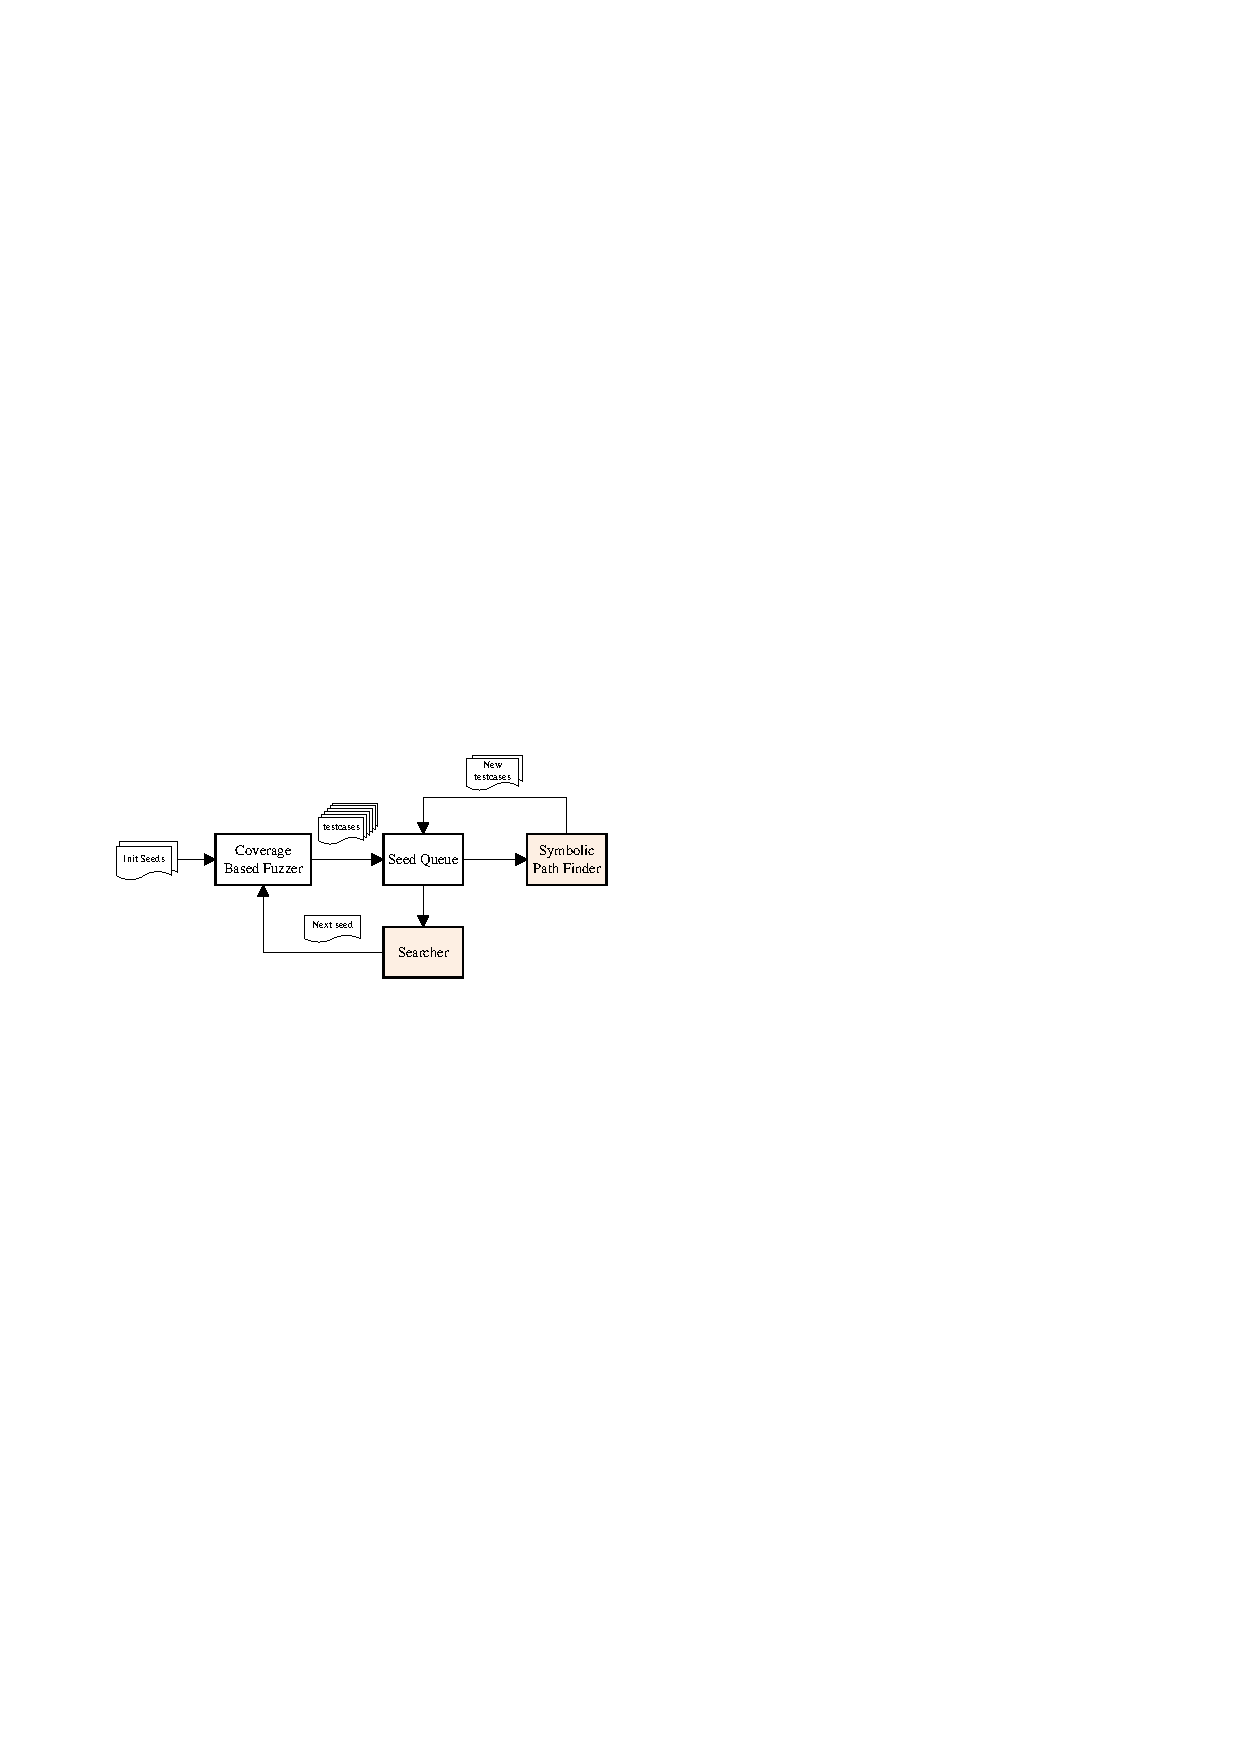
\includegraphics[width=0.7\textwidth]{figures/framework.pdf} 
\caption{High Level Framework.}\label{Framework}
\end{figure}

%TODO: Change this whole part (including the figure)
Figure~\ref{Framework} shows the basic framework of our system. From a high-level scope, our method is built on top of a coverage based fuzzer. The fuzzer accepts some initial seed files as inputs and produces a seed queue by collecting the mutated test cases that trigger new behaviors of the target program. Our main contributions, which consists of two components, namely \emph{Seacher} and \emph{Concolic Path Finder}, focus on improving the quality of the seed queue. Traditional coverage based fuzz testing will pick up seed files from the seed queue one by one as the new seed file to mutate. However, this strategy faces the efficiency problem when testing modern software that have a huge state space. This means the test case will be very huge and mutating each test case in the queue will consumes lots of time. The \emph{Searcher} is designed to select the most promising seed file from the seed queue based on the distance measurement. The most promising seed file is the seed file that has the longest average \textit{distance} from all other seed files in the queue. By doing this, the fuzzer will touch more virgin code areas to improve the coverage as soon as possible in a time budget. The \emph{Concolic Path Finder} is leveraged to help the fuzzer to dive into deeper code areas that guarded by complex path constraints. This is achieved by solving the uncovered branches along with the seed files in the queue. All the test cases generated by \emph{Concolic Path Finder} will be added to the seed queue to find more paths.
